\documentclass{ximera}[font=12pt]

%Next 2 lines create spaces between items in itemize and enumerate
\setitemize{itemsep=1.5ex}
\setenumerate{itemsep=1.5ex}

%Creates space between paragraphs - Maybe???
\setlength{\parskip}{\medskipamount}


\title{Adding Integers: Numberline}    % Use xmlatex all -s to compile when SERVE refuses to work.
\author{Kelly Stady}
\license{CC: 0}                        % replace with an appropriate license, or set it in xmPreamble

\begin{document}

\begin{abstract}

\end{abstract}

\maketitle
\label{xim:AddIntNumLActivity}


\section*{Adding Integers on a Number Line}

Another way to visualize addition is to add on a number line.  

\begin{procedure}[\textbf{Steps for Adding Integers on a Numberline}]

\begin{enumerate}
\item Locate the first number on the number line.

\item If the second number is \textbf{positive}, move to the \textbf{right} that many units.

\item If the second number is \textbf{negative}, take the absolute value of the number and move to the \textbf{left} that many units.
\end{enumerate}
\end{procedure}


\begin{example}

Use a numberline to find the sum $3+7.$ 

\begin{explanation}

Start at $3,$ then move $7$ units to the \textbf{right}.  Movement is to the right, since a \textbf{positive} number is added to $3.$

\begin{center}
\begin{tikzpicture}[x=0.75cm,>=latex, scale=1.5] % Use latex arrowhead style
\draw[thick, <->] (-6,0)--(11,0); % Number line from -6 to 11
\foreach \x in {-5,...,10}
\draw[shift={(\x,0)},color=black] (0pt,2pt) -- (0pt,-2pt) node[below] {\footnotesize $\x$};
\fill (3,0) circle (1.8pt);
\draw[->,out=60,in=120,color=glaucous, thick] (3,0) to (4,0) to (5,0) to (6,0) to (7,0) to (8,0) to (9,0) to (10,0); % Curves
\node[color=OliveGreen!90!black] at (3,-0.65) {\large \textbf{Start}};
\node[color=orange!80!black] at (10,-0.65) {\large \textbf{Stop}};
\node at (6.5,0.9) {$\mathbf{3 + 7 = 10}$};
\end{tikzpicture}
\xmalt{Horizontal number line from negative 5 to 10, with tick marks and labels for each integer.  There is a solid black dot at 3.  
The word ``Start'' is written below the number 3 in green.  A series of connected, blue arches move rightward from 3, landing 
on each integer until stopping with a right-pointing arrow at 10.  The word ``Stop'' is written below the number 10 in orange. 
The equation ''3 plus 7 equals 10'' is displayed centered above the arches.}

\end{center}
\end{explanation}
\end{example}

\begin{example}

Use a numberline to find the sum $3+(-7).$ 

\begin{explanation}

Start at $3$ then move $|-7| = 7$ units to the \textbf{left}.  Movement is to the left, since a \textbf{negative} number is added to $3.$

\begin{center}
\begin{tikzpicture}[x=0.75cm,>=latex, scale=1.5] % Use latex arrowhead style
    \draw[thick, <->] (-6,0)--(11,0); % Number line from -6 to 11
    \foreach \x in {-5,...,10}
    \draw[shift={(\x,0)},color=black] (0pt,2pt) -- (0pt,-2pt) node[below] {\footnotesize $\x$}; % Tick marks for numbers
    \fill (3,0) circle (1.8pt); % Mark start at 3
    % Movement humps from 3 to -4
    \draw[<-,out=60,in=120,color=glaucous, thick] (-4,0) to (-3,0) to (-2,0) to (-1,0) to (0,0) to (1,0) to (2,0) to (3,0); % Curves
    \node[color=OliveGreen!90!black] at (3,-0.65) {\large \textbf{Start}};
    \node[color=orange!80!black] at (-4,-0.65) {\large \textbf{Stop}};
    \node at (-0.5,0.9) {$\mathbf{3 + (-7) = -4}$}; % Label for the operation
\end{tikzpicture}

\xmalt{Horizontal number line from negative 5 to 10, with tick marks and labels for each integer.  There is a solid black dot at 3.  The word ``Start'' is written below the number 3 in green.  
A series of connected, blue arches move leftward from 3, landing on each integer until stopping with a left-pointing arrow at negative 4.  
The word ``Stop'' is written below the number negative 4 in orange.  The equation ``3 plus negative 7 equals negative 4'' is displayed 
centered above the arches.}
\end{center}

\end{explanation}
\end{example}


\begin{problem}
Add using the number line shown below.

\[ -2 + 3 = \answer{1}\]

\begin{center}
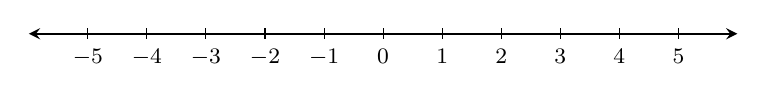
\begin{tikzpicture}[x=0.75cm,>=stealth]
        \draw[thick, <->] (-6,0)--(6,0);
        \foreach \x in {-5,...,5}
        \draw[shift={(\x,0)},color=black] (0pt,2pt) -- (0pt,-2pt) node[below] {\footnotesize $\x$};
\end{tikzpicture}
\xmalt{Horizontal number line from $-5$ to 5, with tick marks and labels for each integer.}
\end{center}
\end{problem}


\begin{problem}
Add using the number line shown below.

\[ -12 + (-3) = \answer{-15} \]


\begin{center} 
  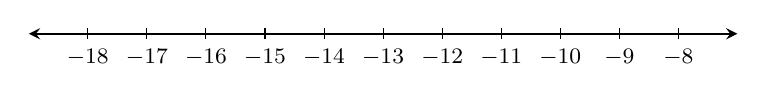
\begin{tikzpicture}[x=0.75cm,>=stealth] 
    % The line spans symmetrically from -6 to 6 around 0 so numberline is centered on html
    \draw[thick, <->] (-6,0) -- (6,0); 
    
    % Maps -18 to the left edge (-5) all the way to -8 at the right edge (+5)
    \foreach \x/\label in {-5/-18, -4/-17, -3/-16, -2/-15, -1/-14, 0/-13, 1/-12, 2/-11, 3/-10, 4/-9, 5/-8} 
      \draw[shift={(\x,0)}, color=black] (0pt,2pt) -- (0pt,-2pt) node[below] {\footnotesize $\label$}; 
  \end{tikzpicture}
  \xmalt{Horizontal number line from negative 18 to negative 8, with tick marks and labels for each integer spanning the full width.} 
\end{center}


\end{problem}


\begin{problem}
Add using the number line shown below.

\[ -1 + 4 =\answer{3} \]

\begin{center}
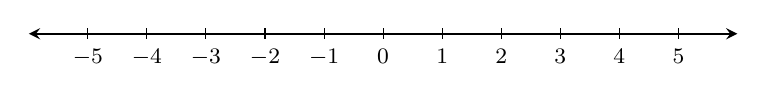
\begin{tikzpicture}[x=0.75cm,>=stealth]
        \draw[thick, <->] (-6,0)--(6,0);
        \foreach \x in {-5,...,5}
        \draw[shift={(\x,0)},color=black] (0pt,2pt) -- (0pt,-2pt) node[below] {\footnotesize $\x$};
\end{tikzpicture}
\xmalt{Horizontal number line from negative 5 to 5, with tick marks and labels for each integer.}
\end{center}
\end{problem}


\begin{problem}
Does the answer to the previous problem change if you switch the order of the numbers and find the value of $4 + (-1)?$

\begin{multipleChoice}
\choice[correct]{No}
\choice{Yes}
\end{multipleChoice}

\begin{feedback}[correct]
That's right, the answer does NOT change!  This is due to a property of addition called the Commutative Property.  
The \textbf{Commutative Property of Addition} states that numbers can be added in any order and the result will be the same.  Therefore, $-1 + 4 = 4 + (-1).$
\end{feedback}

\end{problem}

\end{document}

